\documentclass[misc, color=UCLburgundy, margin=1cm]{uclposter}

\newcommand{\boldf}{\bm{f}}
\newcommand{\boldmu}{\bm{\mu}}
\newcommand{\boldalpha}{\bm{\alpha}}
\newcommand{\boldr}{\bm{r}}
\newcommand{\boldt}{\bm{t}}
\newcommand{\boldg}{\bm{g}}
\newcommand{\boldtheta}{\bm{\theta}}

% Warping operators
\newcommand{\MPWarp}{\tilde{\mathcal{W}}}
\newcommand{\Warp}{\mathcal{W}}

% Others
\newcommand{\etal}{\textit{et al.}~}
\newcommand{\ie}{i.e., }
\newcommand{\eg}{e.g., }

\usepackage{bm}
\usepackage{algorithm}
\usepackage{algorithmic}
\usepackage{caption}
\usepackage{blindtext}
\usepackage{siunitx}

\usepackage[acronym, nomain]{glossaries}

% Define "long-s" key: 
\glsaddkey* {longs}% key 
{\glsentrylong{\glslabel}s}% default value 
{\glsentrylongs}% command analogous to \glsentrytext 
{\Glsentrylongs}% command analogous to \Glsentrytext 
{\glslongs}% command analogous to \glstext 
{\Glslongs}% command analogous to \Glstext 
{\GLSlongs}% command analogous to \GLStext

%% Define "short-s" key: 
\glsaddkey* {shorts}% key 
{\glsentryshort{\glslabel}s}% default value 
{\glsentryshorts}% command analogous to \glsentrytext 
{\Glsentryshorts}% command analogous to \Glsentrytext 
{\glsshorts}% command analogous to \glstext 
{\Glsshorts}% command analogous to \Glstext 
{\GLSshorts}% command analogous to \GLStext

\DeclareRobustCommand{\glss}[1]
{%
  \ifglsused{#1}{\glsshorts{#1}}{\glslongs{#1} (\glsshorts{#1})\glsunset{#1}}%
}

\DeclareRobustCommand{\Glss}[1]
{%
  \ifglsused{#1}{\Glsshorts{#1}}{\Glslongs{#1} (\glsshorts{#1})\glsunset{#1}}%
}

\newacronym{18F-FDG}{18F-FDG}{Fluorine-18 Fludeoxyglucose}
\newacronym{1D}{1D}{1-Dimensional}
\newacronym{2D}{2D}{2-Dimensional}
\newacronym{3D}{3D}{3-Dimensional}
\newacronym[longs={3-Dimensional Point Clouds}, shorts={3DPCs}]{3DPC}{3DPC}{3-Dimensional Point Cloud}
\newacronym{4D}{4D}{4-Dimensional}
% \newacronym{4DCT}{4DCT}{4-Dimensional Computed Tomography}
\newacronym{4DCT}{4DCT}{4D Computed Tomography}
\newacronym{AC}{AC}{Attenuation Corrected}
\newacronym{AD}{AD}{Affine Deformation}
\newacronym{AP}{AP}{Anterior Posterior}
\newacronym{ATP}{ATP}{Adenosine Triphosphate}
% \newacronym{AV-CCT}{AV-CCT}{Averaged CINE-Computed Tomography}
\newacronym{AV-CCT}{AV-CCT}{Averaged CINE-CT}
\newacronym{BE}{BE}{Bending Energy}
\newacronym{BFGS}{BFGS}{Broyden Fletcher Goldfarb Shanno}
\newacronym{CC}{CC}{Correlation Coefficient}
% \newacronym{CCT}{CCT}{CINE-Computed Tomography}
\newacronym{CCT}{CCT}{CINE-CT}
\newacronym{CG}{CG}{Conjugate Gradient}
\newacronym{COM}{COM}{Centre of Mass}
\newacronym[longs={Control Points}, shorts={CPs}]{CP}{CP}{Control Point}
\newacronym[longs={Control Point Grids}, shorts={CPGs}]{CPG}{CPG}{Control Point Grid}
\newacronym{CT}{CT}{Computed Tomography}
\newacronym{DDG}{DDG}{Data Driven Gating}
\newacronym{DD-PCA}{DD-PCA}{Data Driven Principal Component Analysis Surrogate Signal Extraction}
\newacronym{DD}{DD}{Data Driven}
\newacronym[longs={Deformation Vector Fields}, shorts={DVFs}]{DVF}{DVF}{Deformation Vector Field}
\newacronym{EANM}{EANM}{European Association of Nuclear Medicine}
\newacronym{EM}{EM}{Expectation Maximisation}
\newacronym{FDG}{FDG}{Fluorodeoxyglucose}
\newacronym{FFT}{FFT}{Fast Fourier Transform}
\newacronym[longs={Fields of View}, shorts={FOVs}]{FOV}{FOV}{Field Of View}
\newacronym{FWHM}{FWHM}{Full Width at Half Maximum}
\newacronym{GAN}{GAN}{Generative Adversarial Networks}
\newacronym{GD}{GD}{Gradient Descent}
\newacronym{GE}{GE}{General Electric}
\newacronym{GT}{GT}{Ground Truth}
\newacronym{HU}{HU}{Hounsfield Unit}
\newacronym[longs={Image Registrations}, shorts={IRs}]{IR}{IR}{Image Registration}
\newacronym{KBq/mL}{KBq/mL}{Kilo Becquerel per Millilitre}
\newacronym{KeV}{KeV}{Kilo Electron Volt}
\newacronym{KRG}{KRG}{Kinetic Respiratory Gating}
\newacronym{KV}{KV}{Kilo Volt}
\newacronym{L-BFGS-B}{L-BFGS-B}{Low memory Broyden Fletcher Goldfarb Shanno Bounded}
\newacronym{L-BFGS}{L-BFGS}{Low memory Broyden Fletcher Goldfarb Shanno}
\newacronym[longs={Light Emitting Diodes}, shorts={LEDs}]{LED}{LED}{Light Emitting Diode}
\newacronym{LE}{LE}{Linear Energy}
\newacronym{LR}{LR}{Linear Regression}
\newacronym[longs={Lines of Response}, shorts={LORs}]{LOR}{LOR}{Line of Response}
\newacronym{MAE}{MAE}{Mean Absolute Error}
\newacronym{MAD}{MAD}{Median Absolute Difference}
\newacronym{MAPE}{MAPE}{Mean Absolute Percentage Error}
\newacronym{MBF}{MBF}{Myocardial Blood Flow}
\newacronym{MCIR}{MCIR}{Motion Compensated Image Reconstruction}
\newacronym[longs={Motion Compensated Images}, shorts={MCIs}]{MCI}{MCI}{Motion Compensated Image}
\newacronym{MC}{MC}{Motion Correction}
\newacronym{MIC}{MIC}{Medical Imaging Convention}
\newacronym{MI}{MI}{Mutual Information}
\newacronym{ML}{ML}{Maximum Likelihood}
\newacronym{MLAA}{MLAA}{Maximum Likelihood Reconstruction of Activity and Attenuation}
\newacronym{MLE}{MLE}{Maximum Likelihood Estimation}
\newacronym{MLEM}{MLEM}{Maximum Likelihood Expectation Maximisation}
\newacronym[longs={Motion Models}, shorts={MMs}]{MM}{MM}{Motion Model}
\newacronym{MPI}{MPI}{Myocardial Perfusion Imaging}
\newacronym{MR}{MR}{Magnetic Resonance}
\newacronym{MSc}{MSc}{Master of Science}
\newacronym{MSE}{MSE}{Mean Squared Error}
\newacronym[longs={Attenuation Maps}, shorts={Mu-Maps}]{Mu-Map}{Mu-Map}{Attenuation Map}
\newacronym{NAC}{NAC}{Non-Attenuation Corrected}
\newacronym{NMI}{NMI}{Normalised Mutual Information}
\newacronym{ND}{ND}{n-Dimensional}
\newacronym{NMC}{NMC}{Non-Motion Corrected}
\newacronym{NN}{NN}{Neural Network}
\newacronym{NRD}{NRD}{Non-Rigid Deformation}
\newacronym{NTOF}{NTOF}{Non-Time-of-Flight}
\newacronym{OSEM}{OSEM}{Ordered Subset Expectation Maximisation}
\newacronym[longs={Principal Components}, shorts={PCs}]{PC}{PC}{Principal Component}
\newacronym{PCA}{PCA}{Principal Component Analysis}
\newacronym{PCC}{PCC}{Pearson Correlation Coefficient}
\newacronym{PET}{PET}{Positron Emission Tomography}
\newacronym{PLL}{PLL}{Poisson Log Likelihood}
\newacronym{PSD}{PSD}{Power Spectral Density}
\newacronym{PSMA}{PSMA}{Prostate Specific Membrane Antigen}
\newacronym{RANSAC}{RANSAC}{Random Sample Consensus}
\newacronym{RCM}{RCM}{Respiratory Correspondence Model}
\newacronym{RD}{RD}{Rigid Deformation}
\newacronym{RDP}{RDP}{Relative Difference Prior}
\newacronym{RM}{RM}{Respiratory Motion}
\newacronym{RMC}{RMC}{Respiratory Motion Correction}
\newacronym{RMSE}{RMSE}{Root Mean Square Error}
\newacronym[longs={Regions of Interest}, shorts={ROIs}]{ROI}{ROI}{Region of Interest}
\newacronym{RPM}{RPM}{Real Time Position Management}
\newacronym{RTPM}{RTPM}{Real Time Position Management}
\newacronym{SAM}{SAM}{Spectral Analysis Method}
\newacronym{SGD}{SGD}{Stochastic Gradient Descent}
\newacronym{SI}{SI}{Superior Inferior}
\newacronym{SIRF}{SIRF}{Synergistic Image Reconstruction Framework}
\newacronym{SNR}{SNR}{Signal to Noise Ratio}
\newacronym[longs={Surrogate Signals}, shorts={SSs}]{SS}{SS}{Surrogate Signal}
\newacronym{SSD}{SSD}{Sum of Squared Differences}
\newacronym{STFT}{STFT}{Short-time Fourier transform}
\newacronym{STIR}{STIR}{Software for Tomographic Image Reconstruction}
\newacronym{SUV}{SUV}{Standard Uptake Value}
\newacronym{SVD}{SVD}{Singular Value Decomposition}
\newacronym{TOF}{TOF}{Time-of-Flight}
\newacronym{TPS}{TPS}{Thin Plate Spline}
\newacronym{XCAT}{XCAT}{4-Dimensional Extended Cardiac Torso}

\glsunset{18F-FDG}
\glsunset{1D}
\glsunset{2D}
\glsunset{3D}
\glsunset{4D}
\glsunset{4DCT}
\glsunset{ATP}
\glsunset{BFGS}
\glsunset{CT}
\glsunset{EANM}
\glsunset{FDG}
\glsunset{GE}
\glsunset{L-BFGS-B}
\glsunset{L-BFGS}
\glsunset{LED}
\glsunset{MIC}
\glsunset{MLAA}
\glsunset{MLEM}
\glsunset{MR}
\glsunset{MSc}
\glsunset{Mu-Map}
\glsunset{NTOF}
\glsunset{OSEM}
\glsunset{PCA}
\glsunset{PET}
\glsunset{RANSAC}
\glsunset{RPM}
\glsunset{RTPM}
\glsunset{SIRF}
\glsunset{STIR}
\glsunset{SUV}
\glsunset{TOF}
\glsunset{XCAT}

\usepackage[style=ieee, maxbibnames=1, minbibnames=1, maxcitenames=1, mincitenames=1, backend=biber, defernumbers=false]{biblatex}
\addbibresource{./Biblio.bib}

\AtEveryBibitem{\clearfield{month}}
\AtEveryBibitem{\clearfield{day}}
\AtEveryBibitem{\clearfield{volume}}
\AtEveryBibitem{\clearfield{issue}}
\AtEveryBibitem{\clearfield{pages}}
\AtEveryBibitem{\clearfield{number}}
\AtEveryBibitem{\clearfield{title}}
\AtEveryBibitem{\clearfield{isbn}}
\AtEveryBibitem{\clearfield{keywords}}
\AtEveryBibitem{\clearfield{issn}}
\AtEveryBibitem{\clearfield{journal}}

\usepackage{fontspec}
\setmainfont[Ligatures=TeX]{LexendDeca-Regular.ttf}

\begin{document}
    \title{Comparison of Motion Correction Methods Incorporating Motion Modelling for PET/CT Using a Single Breath Hold Attenuation Map}
    
    \author[12*]{Alexander~C.~Whitehead}
    \author[2]{Ander~Biguri}
    \author[3]{Kuan-Hao~Su}
    \author[3]{Scott~D.~Wollenweber}
    \author[3]{Charles~W.~Stearns}
    \author[1]{Brian~F.~Hutton}
    \author[2]{\newline~Jamie~R.~McClelland}
    \author[12]{Kris~Thielemans}
    
    \affil[1]{INM, UCL}
    \affil[2]{CMIC, UCL}
    \affil[3]{GE Healthcare}
    \affil[*]{alexander.whitehead.18@ucl.ac.uk}
    
    \maketitle

    \begin{multicols}{4}
        \normalsize
        
        \section*{Introduction}
            \begin{highlightbox}[UCLlightgreen]
                \begin{itemize}
                    \item \gls{RM} reduces resolution and quantification accuracy in \gls{PET}.
                    \item A \gls{MM} is a \gls{MC} technique where a \glss{DVF} is parametrised by a \gls{SS}~\cite{McClelland2013}.
                    \item A \gls{MM} is more robust to noise and allows for correction of unseen data.
                    \item This work will demonstrate a comparison of registration methods, including \glss{MM}.
                    \item This work will fix the \gls{Mu-Map} at end inhalation. This is more clinically relevant but also challenging when compared to~\cite{Whitehead2020PET/CTFields}.
                    \item This work differentiates itself by using a \gls{2D} \gls{SS}, and group-wise registration.
                \end{itemize}
            \end{highlightbox}
        
        \section*{Methods}
            \subsection*{\underline{\textbf{XCAT Volume Generation}}}
                \begin{itemize}
                    \item \gls{XCAT} generated 240 volumes using a \SI{120}{\second} respiratory trace.
                    \item Activity concentrations from a static \gls{18F-FDG} patient scan.
                    \item \gls{FOV} including the base of the lungs with a \SI{20}{\milli\metre} diameter lesion.
                \end{itemize}
            
            \subsection*{\underline{\textbf{PET Simulation and Reconstruction}}}
                \begin{itemize}
                    \item Simulated using the geometry of a \gls{GE} Discovery 710.
                    \item Pseudo-randoms and scatter were added.
                    \item A respiratory \gls{SS} was generated using \gls{PCA}~\cite{Thielemans2011}.
                    \item Gated into 30 respiratory bins using displacement gating (10 amplitude and three gradient bins).
                    \item Reconstructed without \gls{AC} using \gls{OSEM} with two full iterations and 24 subsets.
                \end{itemize}
            
            \subsection*{\underline{\textbf{Registration}}}
                \begin{itemize}
                    \item Pre-processing including; replication of end-slices and Yeo-Johnson transform.
                    \item Two registration methods were used; pair-wise (reference position selected as the gate with the highest number of counts) and group-wise registration (initial pair-wise step).
                    \item NiftyReg used to perform B-spline registrations.
                    \item \acrlong{CPG} spacing, \acrlong{BE} weight and number of iterations tuned using a grid search.
                \end{itemize}
            
            \subsection*{\underline{\textbf{Motion Model Estimation}}}
                \begin{itemize}
                    \item \gls{MM} fit as a direct \acrlong{RCM} on registration \glss{DVF} using \gls{SS}.
                    \item Weighted \acrlong{LR} on total counts in gate.
                    \item For group-wise registration, \gls{MM} fit between each iteration.
                \end{itemize}
            
            \subsection*{\underline{\textbf{Attenuation Map Warping}}}
                \begin{itemize}
                    \item \gls{Mu-Map} at end inhalation selected.
                    \item \gls{MC} \gls{PET} volume registered to \gls{Mu-Map}.
                    \item Resulting \glss{DVF} composed.
                    \item Inverse \glss{DVF} used to warp \gls{Mu-Map} to each gate.
                \end{itemize}
            
            \subsection*{\underline{\textbf{Image Reconstruction with AC}}}
                \begin{itemize}
                    \item Data re-reconstructed with \gls{AC} and \gls{MC} reapplied as above.
                    \item Volumes post-filtered with a Gaussian smoothing, (\gls{FWHM} of \SI{6.39}{\milli\metre} in transverse plane and \SI{3.27}{\milli\metre} in the axial direction).
                \end{itemize}
            
            \subsection*{\underline{\textbf{Evaluation}}}
                \begin{highlightbox}[UCLlightgreen]
                    \begin{itemize}
                        \item Data also reconstructed without \gls{MC}, using either a sum of all \glss{Mu-Map} or the end inhalation \gls{Mu-Map}.
                        \item Volumes without \gls{MC} registered to the position of the \gls{Mu-Map}.
                        \item \glss{DVF} generated by each method were also applied to noiseless data for visual analysis.
                        \item Comparisons used included; a profile over the lesion, \gls{SUV}\textsubscript{max} and \gls{SUV}\textsubscript{peak}.
                    \end{itemize}
                \end{highlightbox}
        
        \section*{Results}
            \begin{figure}[H]
                \centering
                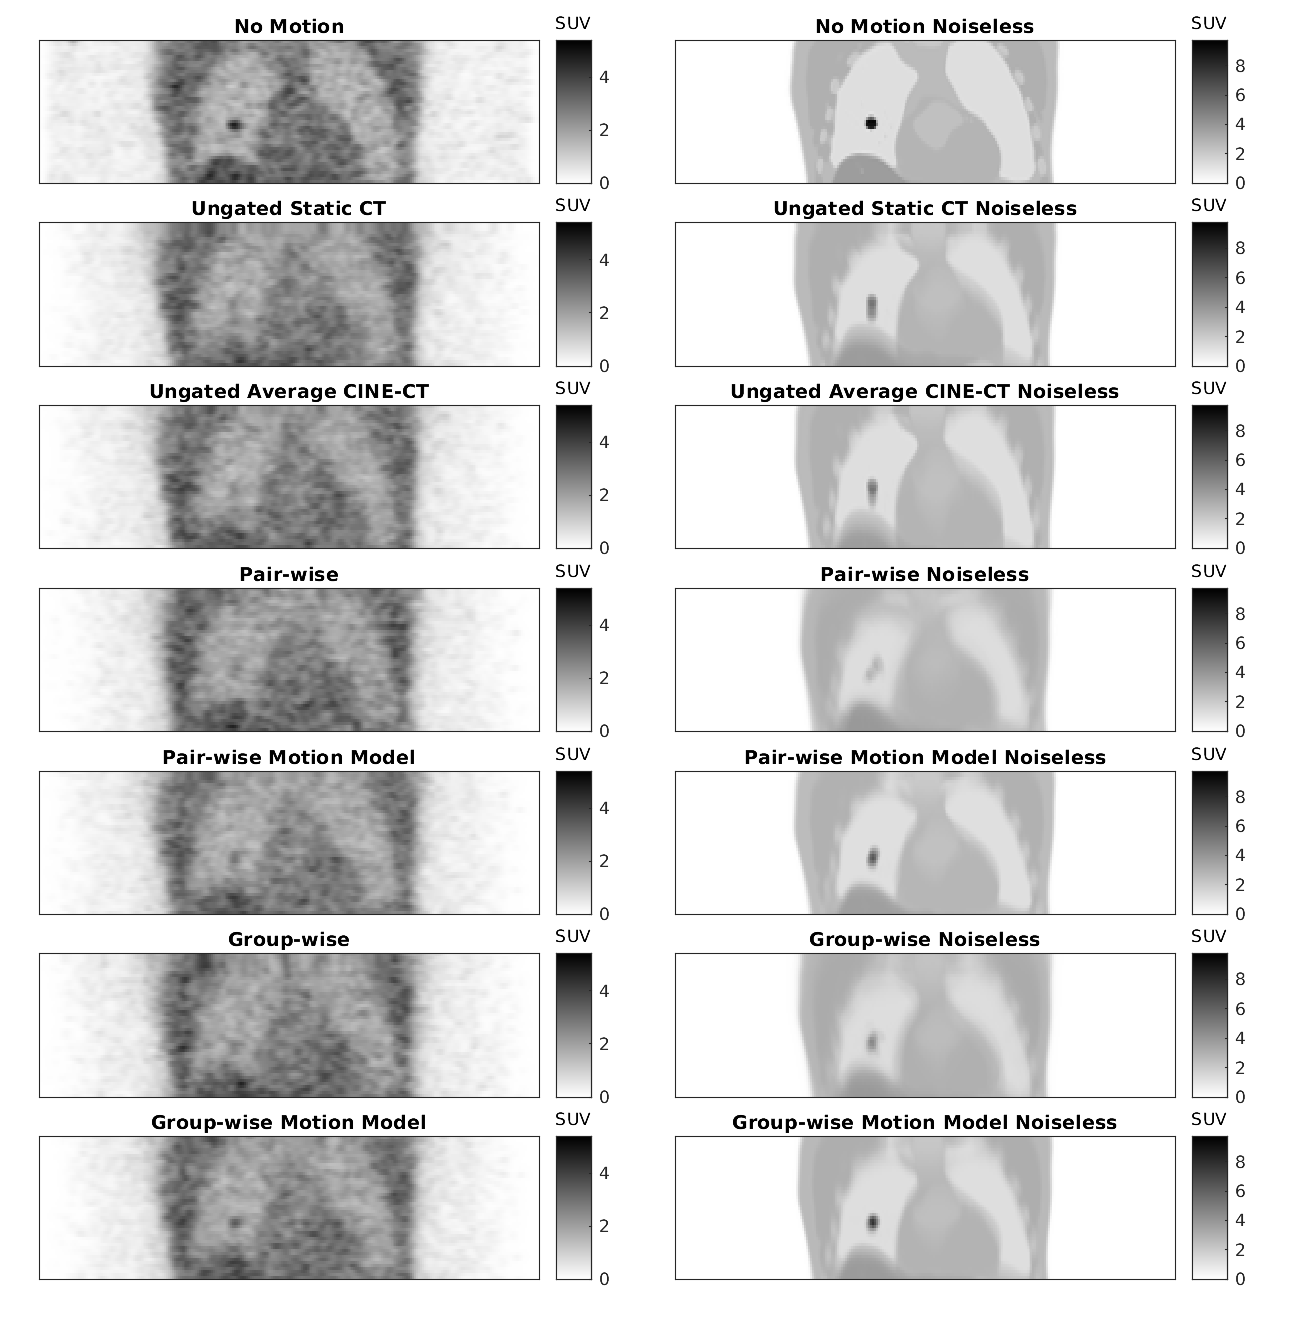
\includegraphics[width=0.9\linewidth]{visual_analysis.png}
                \begin{highlightbox}[UCLlightblue]
                    \captionsetup{singlelinecheck=false, justification=centering}
                    \caption{First column \gls{AC} \gls{MC} reconstructions, second column noiseless data; ungated static \gls{CT}, ungated \gls{AV-CCT}, pair-wise, pair-wise \gls{MM}, group-wise, group-wise \gls{MM}. Colour map ranges consistent for all images in each column.}
                \end{highlightbox}
            \end{figure}
            
            \begin{figure}[H]
                \centering
                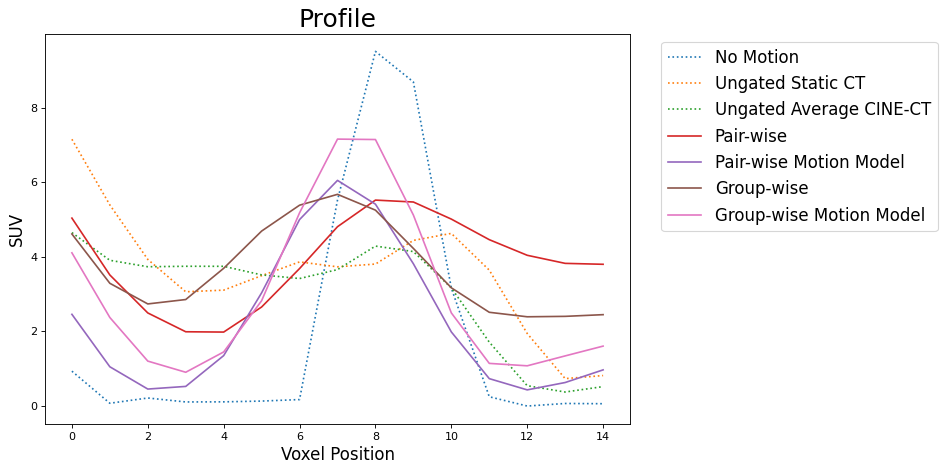
\includegraphics[width=0.9\linewidth]{profile.png}
                \begin{highlightbox}[UCLlightblue]
                    \captionsetup{singlelinecheck=false, justification=centering}
                    \caption{A profile across the lesion for; ungated static \gls{CT}, ungated \gls{AV-CCT}, pair-wise, pair-wise \gls{MM}, group-wise, group-wise \gls{MM}.}
                \end{highlightbox}
            \end{figure}
            
            \begin{table}[H]
                \centering
                \begin{highlightbox}[UCLlightblue]
                    \captionsetup{singlelinecheck=false, justification=centering}
                    \caption{Comparison of \gls{SUV}\textsubscript{max} and \gls{SUV}\textsubscript{peak} between: ungated static \gls{CT}, ungated \gls{AV-CCT}, pair-wise, pair-wise \gls{MM}, group-wise, group-wise \gls{MM}.}
                \end{highlightbox}
                \vspace{1.0cm}
                \resizebox*{0.75\linewidth}{!}
                {
                    \begin{tabular}{||c|cc||}
                        \hline
                        \textbf{\gls{SUV}}                  & \textbf{Max}  & \textbf{Peak} \\
                        \hline
                        \textbf{No Motion}                  & 9.50        & 9.06 \\
                        \hline
                        \textbf{Ungated Static \gls{CT}}    & 5.25        & 5.15 \\
                        \textbf{Ungated \gls{AV-CCT}}       & 5.38        & 5.07 \\
                        \hline
                        \textbf{Pair-wise}                  & 4.21        & 3.92 \\
                        \textbf{Pair-wise \gls{MM}}         & 6.63        & 6.07 \\
                        \hline
                        \textbf{Group-wise}                 & 4.42        & 4.21 \\
                        \textbf{Group-wise \gls{MM}}        & 7.64        & 7.03 \\
                        \hline
                    \end{tabular}
                }
            \end{table}
        
        \section*{Conclusion}
            \begin{itemize}
                \item Adding a \gls{MM} to any \gls{MC} method improved the quality of volumes produced.
                \item For \gls{MC} to be successful, for very noisy data, \glss{MM} are almost required.
                \item Future work will focus on testing on patient data and incorporating the method into an iterative \acrlong{IR} and \gls{MC} method.
            \end{itemize}
        
        \AtNextBibliography{\small}
        \printbibliography
        
        \small
        \section*{Acknowledgements}
            \begin{itemize}
                \item This research is supported by GE Healthcare, the NIHR UCLH Biomedical Research Centre and the UCL EPSRC Centre for Doctoral Training in Intelligent, Integrated Imaging in Healthcare (i4health) grant (EP/L016478/1).
                \item The software used was partly produced by the Computational Collaborative Project on Synergistic Biomedical Imaging, CCP SyneRBI, UK EPSRC grant (EP/T026693/1).
                \item Jamie~R.~McClelland is supported by a Cancer Research UK Centres Network Accelerator Award grant (A21993) to the ART-NET consortium and a CRUK Multi-disciplinary grant (CRC 521).
            \end{itemize}
    \end{multicols}
\end{document}
